\documentclass[border=4pt]{standalone}
\usepackage[T1]{fontenc}
\usepackage{lmodern}
\usepackage{amsmath}
\usepackage{pgfplots}
\pgfplotsset{compat=1.18}
\usepgfplotslibrary{groupplots,fillbetween}
\usetikzlibrary{calc,arrows.meta}
% one colour per kind of method, the same in every figure (Okabe-Ito)
\definecolor{neur}{HTML}{D55E00}   % neurons chosen by attribution
\definecolor{dirc}{HTML}{009E73}   % directions from the weird-vs-normal contrast
\definecolor{read}{HTML}{0072B2}   % readout methods and interventions chosen from readouts
\definecolor{pers}{HTML}{CC79A7}   % Assistant Axis / persona
\definecolor{ctrl}{HTML}{8C8C8C}   % random controls
\definecolor{meas}{HTML}{E69F00}   % measured outcome
\definecolor{ink}{HTML}{222222}
\pgfplotsset{
  every axis/.append style={clip=false, font=\small, axis line style={black!55}, tick style={black!55}, tick align=outside,
    label style={font=\small}, tick label style={font=\footnotesize}, title style={font=\small, align=center}},
  grid style={black!9, line width=0.4pt},
  every axis legend/.append style={font=\footnotesize, draw=none, fill=none},
  ci/.style={/pgfplots/error bars/x dir=both, /pgfplots/error bars/x explicit, /pgfplots/error bars/error bar style={line width=0.8pt}, /pgfplots/error bars/error mark=none},
  yci/.style={/pgfplots/error bars/y dir=both, /pgfplots/error bars/y explicit, /pgfplots/error bars/error bar style={line width=0.8pt}, /pgfplots/error bars/error mark=none},
}

\begin{document}
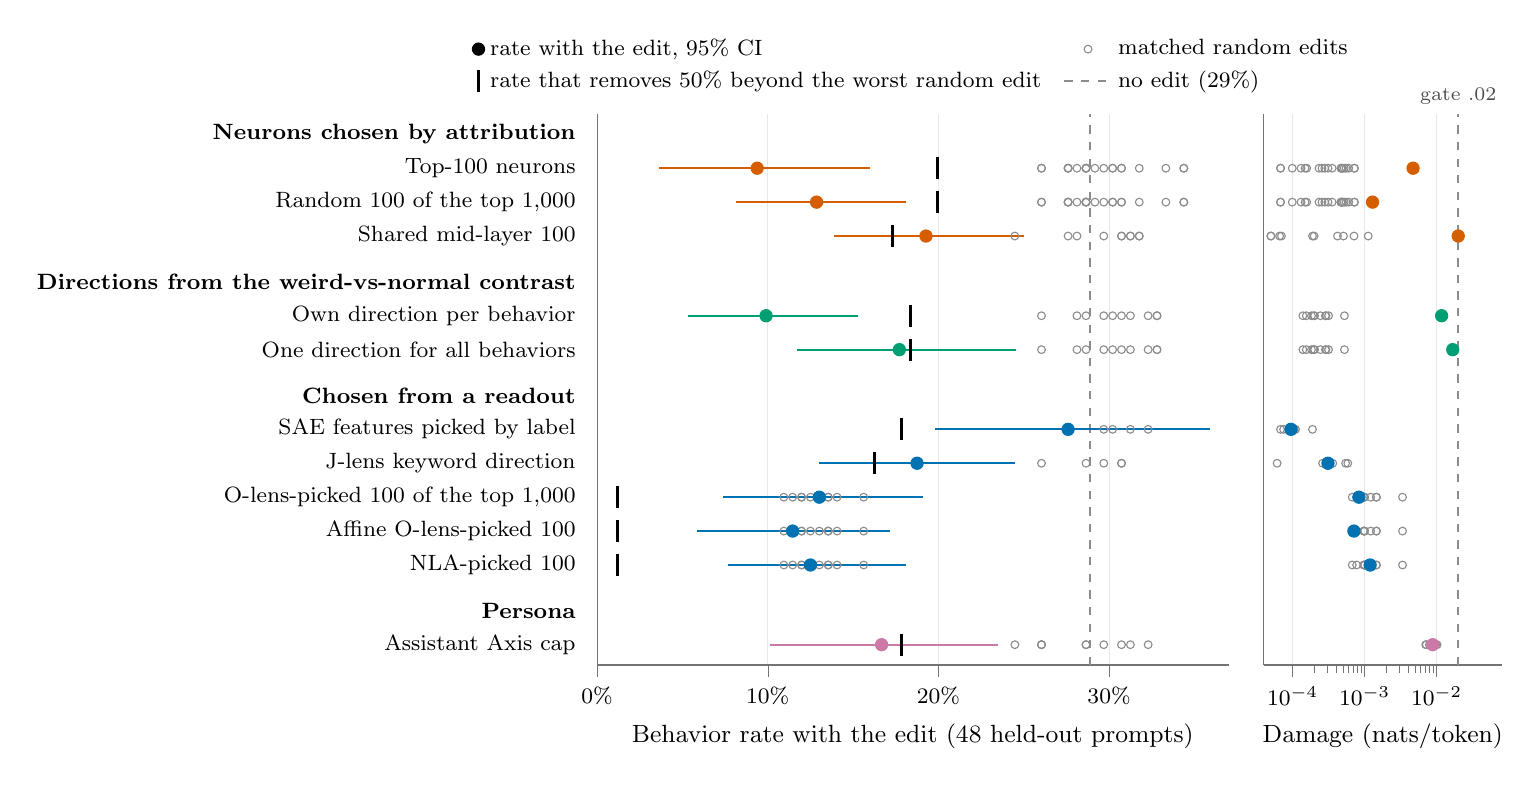
\begin{tikzpicture}
\begin{groupplot}[group style={group size=2 by 1, horizontal sep=0.45cm, y descriptions at=edge left}, height=8.58cm, ymin=-15.65, ymax=0.6, ytick={0.00,-1.00,-2.00,-3.00,-4.35,-5.35,-6.35,-7.70,-8.70,-9.70,-10.70,-11.70,-12.70,-14.05,-15.05}, yticklabels={{\textbf{Neurons chosen by attribution}},{Top-100 neurons},{Random 100 of the top 1,000},{Shared mid-layer 100},{\textbf{Directions from the weird-vs-normal contrast}},{Own direction per behavior},{One direction for all behaviors},{\textbf{Chosen from a readout}},{SAE features picked by label},{J-lens keyword direction},{O-lens-picked 100 of the top 1,000},{Affine O-lens-picked 100},{NLA-picked 100},{\textbf{Persona}},{Assistant Axis cap}}, y tick label style={font=\footnotesize}, major y tick style={draw=none}, axis y line*=left, axis x line*=bottom, xmajorgrids]
\nextgroupplot[width=9.6cm, xmin=0, xmax=37, xtick={0,10,20,30}, xticklabel={$\pgfmathprintnumber{\tick}\%$}, xlabel={Behavior rate with the edit (48 held-out prompts)}, legend style={at={(0.5,1.02)}, anchor=south, legend columns=2, /tikz/every even column/.append style={column sep=6pt}}, legend cell align=left]
\draw[black!45, dashed, line width=0.7pt] (axis cs:28.91,-15.65) -- (axis cs:28.91,0.6);
\addlegendimage{only marks, mark=*, mark size=2.2pt, black}\addlegendentry{rate with the edit, 95\% CI}
\addlegendimage{only marks, mark=o, mark size=1.4pt, ctrl}\addlegendentry{matched random edits}
\addlegendimage{only marks, mark=|, mark size=4pt, line width=1.1pt, black}\addlegendentry{rate that removes 50\% beyond the worst random edit}
\addlegendimage{dashed, black!45, line width=0.7pt}\addlegendentry{no edit (29\%)}
\addplot[only marks, mark=o, mark size=1.4pt, ctrl, forget plot] coordinates {(30.21,-1.00) (26.04,-1.00) (28.12,-1.00) (28.65,-1.00) (28.65,-1.00) (28.65,-1.00) (31.77,-1.00) (29.17,-1.00) (30.73,-1.00) (30.21,-1.00) (30.73,-1.00) (27.60,-1.00) (33.33,-1.00) (27.60,-1.00) (28.65,-1.00) (34.38,-1.00) (26.04,-1.00) (27.60,-1.00) (29.69,-1.00) (34.38,-1.00)};
\addplot[only marks, mark=|, mark size=4pt, line width=1.1pt, black, forget plot] coordinates {(19.92,-1.00)};
\addplot[only marks, mark=*, mark size=2.2pt, neur, ci, forget plot] coordinates {(9.38,-1.00) += (6.63,0) -= (5.73,0)};
\addplot[only marks, mark=o, mark size=1.4pt, ctrl, forget plot] coordinates {(30.21,-2.00) (26.04,-2.00) (28.12,-2.00) (28.65,-2.00) (28.65,-2.00) (28.65,-2.00) (31.77,-2.00) (29.17,-2.00) (30.73,-2.00) (30.21,-2.00) (30.73,-2.00) (27.60,-2.00) (33.33,-2.00) (27.60,-2.00) (28.65,-2.00) (34.38,-2.00) (26.04,-2.00) (27.60,-2.00) (29.69,-2.00) (34.38,-2.00)};
\addplot[only marks, mark=|, mark size=4pt, line width=1.1pt, black, forget plot] coordinates {(19.92,-2.00)};
\addplot[only marks, mark=*, mark size=2.2pt, neur, ci, forget plot] coordinates {(12.86,-2.00) += (5.22,0) -= (4.73,0)};
\addplot[only marks, mark=o, mark size=1.4pt, ctrl, forget plot] coordinates {(31.77,-3.00) (29.69,-3.00) (28.12,-3.00) (24.48,-3.00) (30.73,-3.00) (27.60,-3.00) (31.25,-3.00) (30.73,-3.00) (31.77,-3.00) (31.25,-3.00)};
\addplot[only marks, mark=|, mark size=4pt, line width=1.1pt, black, forget plot] coordinates {(17.32,-3.00)};
\addplot[only marks, mark=*, mark size=2.2pt, neur, ci, forget plot] coordinates {(19.27,-3.00) += (5.73,0) -= (5.38,0)};
\addplot[only marks, mark=o, mark size=1.4pt, ctrl, forget plot] coordinates {(32.81,-5.35) (31.25,-5.35) (32.81,-5.35) (29.69,-5.35) (30.21,-5.35) (32.29,-5.35) (28.12,-5.35) (28.65,-5.35) (26.04,-5.35) (30.73,-5.35)};
\addplot[only marks, mark=|, mark size=4pt, line width=1.1pt, black, forget plot] coordinates {(18.36,-5.35)};
\addplot[only marks, mark=*, mark size=2.2pt, dirc, ci, forget plot] coordinates {(9.90,-5.35) += (5.41,0) -= (4.58,0)};
\addplot[only marks, mark=o, mark size=1.4pt, ctrl, forget plot] coordinates {(32.81,-6.35) (31.25,-6.35) (32.81,-6.35) (29.69,-6.35) (30.21,-6.35) (32.29,-6.35) (28.12,-6.35) (28.65,-6.35) (26.04,-6.35) (30.73,-6.35)};
\addplot[only marks, mark=|, mark size=4pt, line width=1.1pt, black, forget plot] coordinates {(18.36,-6.35)};
\addplot[only marks, mark=*, mark size=2.2pt, dirc, ci, forget plot] coordinates {(17.71,-6.35) += (6.82,0) -= (6.01,0)};
\addplot[only marks, mark=o, mark size=1.4pt, ctrl, forget plot] coordinates {(31.25,-8.70) (29.69,-8.70) (30.21,-8.70) (32.29,-8.70) (27.60,-8.70)};
\addplot[only marks, mark=|, mark size=4pt, line width=1.1pt, black, forget plot] coordinates {(17.84,-8.70)};
\addplot[only marks, mark=*, mark size=2.2pt, read, ci, forget plot] coordinates {(27.60,-8.70) += (8.33,0) -= (7.81,0)};
\addplot[only marks, mark=o, mark size=1.4pt, ctrl, forget plot] coordinates {(28.65,-9.70) (30.73,-9.70) (30.73,-9.70) (26.04,-9.70) (29.69,-9.70)};
\addplot[only marks, mark=|, mark size=4pt, line width=1.1pt, black, forget plot] coordinates {(16.28,-9.70)};
\addplot[only marks, mark=*, mark size=2.2pt, read, ci, forget plot] coordinates {(18.75,-9.70) += (5.73,0) -= (5.73,0)};
\addplot[only marks, mark=o, mark size=1.4pt, ctrl, forget plot] coordinates {(15.62,-10.70) (13.54,-10.70) (13.54,-10.70) (11.98,-10.70) (10.94,-10.70) (13.02,-10.70) (14.06,-10.70) (12.50,-10.70) (11.46,-10.70) (11.98,-10.70)};
\addplot[only marks, mark=|, mark size=4pt, line width=1.1pt, black, forget plot] coordinates {(1.17,-10.70)};
\addplot[only marks, mark=*, mark size=2.2pt, read, ci, forget plot] coordinates {(13.02,-10.70) += (6.10,0) -= (5.64,0)};
\addplot[only marks, mark=o, mark size=1.4pt, ctrl, forget plot] coordinates {(15.62,-11.70) (13.54,-11.70) (13.54,-11.70) (11.98,-11.70) (10.94,-11.70) (13.02,-11.70) (14.06,-11.70) (12.50,-11.70) (11.46,-11.70) (11.98,-11.70)};
\addplot[only marks, mark=|, mark size=4pt, line width=1.1pt, black, forget plot] coordinates {(1.17,-11.70)};
\addplot[only marks, mark=*, mark size=2.2pt, read, ci, forget plot] coordinates {(11.46,-11.70) += (5.73,0) -= (5.58,0)};
\addplot[only marks, mark=o, mark size=1.4pt, ctrl, forget plot] coordinates {(15.62,-12.70) (13.54,-12.70) (13.54,-12.70) (11.98,-12.70) (10.94,-12.70) (13.02,-12.70) (14.06,-12.70) (12.50,-12.70) (11.46,-12.70) (11.98,-12.70)};
\addplot[only marks, mark=|, mark size=4pt, line width=1.1pt, black, forget plot] coordinates {(1.17,-12.70)};
\addplot[only marks, mark=*, mark size=2.2pt, read, ci, forget plot] coordinates {(12.50,-12.70) += (5.59,0) -= (4.85,0)};
\addplot[only marks, mark=o, mark size=1.4pt, ctrl, forget plot] coordinates {(28.65,-15.05) (24.48,-15.05) (26.04,-15.05) (30.73,-15.05) (28.65,-15.05) (29.69,-15.05) (26.04,-15.05) (32.29,-15.05) (26.04,-15.05) (31.25,-15.05)};
\addplot[only marks, mark=|, mark size=4pt, line width=1.1pt, black, forget plot] coordinates {(17.84,-15.05)};
\addplot[only marks, mark=*, mark size=2.2pt, pers, ci, forget plot] coordinates {(16.67,-15.05) += (6.83,0) -= (6.56,0)};
\nextgroupplot[width=4.6cm, xmode=log, xmin=4e-5, xmax=0.08, xtick={1e-4,1e-3,1e-2}, xticklabels={$10^{-4}$,$10^{-3}$,$10^{-2}$}, xlabel={Damage (nats/token)}, yticklabels={}]
\draw[black!45, dashed, line width=0.7pt] (axis cs:0.02,-15.65) -- (axis cs:0.02,0.6) node[above, font=\scriptsize, black!70] {gate .02};
\addplot[only marks, mark=o, mark size=1.4pt, ctrl] coordinates {(0.000233,-1.00) (0.000472,-1.00) (0.000068,-1.00) (0.000722,-1.00) (0.000256,-1.00) (0.000068,-1.00) (0.000157,-1.00) (0.000494,-1.00) (0.000311,-1.00) (0.000354,-1.00) (0.000554,-1.00) (0.000485,-1.00) (0.000131,-1.00) (0.000603,-1.00) (0.000149,-1.00) (0.000520,-1.00) (0.000099,-1.00) (0.000469,-1.00) (0.000280,-1.00) (0.000721,-1.00)};
\addplot[only marks, mark=*, mark size=2.2pt, neur] coordinates {(0.004718,-1.00)};
\addplot[only marks, mark=o, mark size=1.4pt, ctrl] coordinates {(0.000233,-2.00) (0.000472,-2.00) (0.000068,-2.00) (0.000722,-2.00) (0.000256,-2.00) (0.000068,-2.00) (0.000157,-2.00) (0.000494,-2.00) (0.000311,-2.00) (0.000354,-2.00) (0.000554,-2.00) (0.000485,-2.00) (0.000131,-2.00) (0.000603,-2.00) (0.000149,-2.00) (0.000520,-2.00) (0.000099,-2.00) (0.000469,-2.00) (0.000280,-2.00) (0.000721,-2.00)};
\addplot[only marks, mark=*, mark size=2.2pt, neur] coordinates {(0.001290,-2.00)};
\addplot[only marks, mark=o, mark size=1.4pt, ctrl] coordinates {(0.000509,-3.00) (0.000066,-3.00) (0.000189,-3.00) (0.000050,-3.00) (0.000421,-3.00) (0.000050,-3.00) (0.000070,-3.00) (0.000713,-3.00) (0.001123,-3.00) (0.000199,-3.00)};
\addplot[only marks, mark=*, mark size=2.2pt, neur] coordinates {(0.019979,-3.00)};
\addplot[only marks, mark=o, mark size=1.4pt, ctrl] coordinates {(0.000196,-5.35) (0.000244,-5.35) (0.000139,-5.35) (0.000291,-5.35) (0.000183,-5.35) (0.000202,-5.35) (0.000525,-5.35) (0.000155,-5.35) (0.000316,-5.35) (0.000286,-5.35)};
\addplot[only marks, mark=*, mark size=2.2pt, dirc] coordinates {(0.011748,-5.35)};
\addplot[only marks, mark=o, mark size=1.4pt, ctrl] coordinates {(0.000196,-6.35) (0.000244,-6.35) (0.000139,-6.35) (0.000291,-6.35) (0.000183,-6.35) (0.000202,-6.35) (0.000525,-6.35) (0.000155,-6.35) (0.000316,-6.35) (0.000286,-6.35)};
\addplot[only marks, mark=*, mark size=2.2pt, dirc] coordinates {(0.016758,-6.35)};
\addplot[only marks, mark=o, mark size=1.4pt, ctrl] coordinates {(0.000189,-8.70) (0.000105,-8.70) (0.000075,-8.70) (0.000068,-8.70) (0.000110,-8.70)};
\addplot[only marks, mark=*, mark size=2.2pt, read] coordinates {(0.000095,-8.70)};
\addplot[only marks, mark=o, mark size=1.4pt, ctrl] coordinates {(0.000545,-9.70) (0.000061,-9.70) (0.000361,-9.70) (0.000261,-9.70) (0.000584,-9.70)};
\addplot[only marks, mark=*, mark size=2.2pt, read] coordinates {(0.000310,-9.70)};
\addplot[only marks, mark=o, mark size=1.4pt, ctrl] coordinates {(0.001216,-10.70) (0.001461,-10.70) (0.003365,-10.70) (0.000997,-10.70) (0.000972,-10.70) (0.000674,-10.70) (0.000996,-10.70) (0.000775,-10.70) (0.001455,-10.70) (0.000989,-10.70)};
\addplot[only marks, mark=*, mark size=2.2pt, read] coordinates {(0.000835,-10.70)};
\addplot[only marks, mark=o, mark size=1.4pt, ctrl] coordinates {(0.001216,-11.70) (0.001461,-11.70) (0.003365,-11.70) (0.000997,-11.70) (0.000972,-11.70) (0.000674,-11.70) (0.000996,-11.70) (0.000775,-11.70) (0.001455,-11.70) (0.000989,-11.70)};
\addplot[only marks, mark=*, mark size=2.2pt, read] coordinates {(0.000711,-11.70)};
\addplot[only marks, mark=o, mark size=1.4pt, ctrl] coordinates {(0.001216,-12.70) (0.001461,-12.70) (0.003365,-12.70) (0.000997,-12.70) (0.000972,-12.70) (0.000674,-12.70) (0.000996,-12.70) (0.000775,-12.70) (0.001455,-12.70) (0.000989,-12.70)};
\addplot[only marks, mark=*, mark size=2.2pt, read] coordinates {(0.001194,-12.70)};
\addplot[only marks, mark=o, mark size=1.4pt, ctrl] coordinates {(0.010154,-15.05) (0.007074,-15.05) (0.008649,-15.05) (0.007197,-15.05) (0.007946,-15.05) (0.008827,-15.05) (0.009749,-15.05) (0.008418,-15.05) (0.008754,-15.05) (0.008650,-15.05)};
\addplot[only marks, mark=*, mark size=2.2pt, pers] coordinates {(0.008826,-15.05)};
\end{groupplot}
\end{tikzpicture}
\end{document}
